\documentclass[areasetadvanced]{scrartcl}

\usepackage[utf8]{inputenc}
\usepackage[T2A]{fontenc}
\usepackage[english,russian]{babel}
\usepackage[footskip=1cm,left=25mm, right=15mm, top=20mm, bottom=20mm]{geometry}
\usepackage{setspace}
\usepackage{amsmath, amssymb}  
\usepackage{graphicx}
\usepackage[final]{pdfpages}
\usepackage{ragged2e}
\usepackage{tikz}
\usetikzlibrary{arrows.meta}
\usepackage{float}
\usepackage{dashrule}
\usepackage{lipsum}
\pagestyle{plain} 
\usepackage{fancyhdr} 
\usepackage{hyperref} 
\usepackage{xcolor}
\usepackage{tikz}
\usetikzlibrary{positioning,arrows.meta}
\usetikzlibrary{arrows.meta,positioning,automata}
\usepackage{listings}
\usepackage{parskip}
\usepackage{textcomp, enumitem}
\usepackage{indentfirst}
\usepackage{graphicx}
\usepackage{pdflscape}
\usepackage{algorithm}
\usepackage{algpseudocode}
\usepackage{array}  
\usepackage{geometry}
\usepackage{tabularx}
\usepackage{afterpage}
\usepackage{minted}
\setcounter{secnumdepth}{3}  
\setcounter{tocdepth}{3}     
\usepackage{listings} 
\setlength{\parindent}{1.25cm}
\tikzstyle{block} = [rectangle, rounded corners, minimum width=3cm, minimum height=1cm, text centered, draw=black, fill=lightgray]

\setkomafont{sectioning}{\normalfont\bfseries} 
\setkomafont{section}{\normalfont\Large\bfseries}
\setkomafont{subsection}{\normalfont\large\bfseries}
\setkomafont{subsubsection}{\normalfont\large\bfseries}
\setkomafont{paragraph}{\normalfont\large\bfseries} 



\lstdefinelanguage{json}{
  basicstyle=\ttfamily\small,
  breaklines=true,
  showstringspaces=false,
  frame=single,
  backgroundcolor=\color{white!6},
  literate=
   *{:}{{{\color{purple}{:}}}}{1}
    {,}{{{\color{purple}{,}}}}{1}
    {\{}{{{\color{red}{\{}}}}{1}
    {\}}{{{\color{red}{\}}}}}{1}
    {[}{{{\color{blue}{[}}}}{1}
    {]}{{{\color{blue}{]}}}}{1}
    {а}{а}{1}
    {б}{б}{1}
    {в}{в}{1}
    {г}{г}{1}
    {д}{д}{1}
    {е}{е}{1}
    {ё}{ё}{1}
    {ж}{ж}{1}
    {з}{з}{1}
    {и}{и}{1}
    {й}{й}{1}
    {к}{к}{1}
    {л}{л}{1}
    {м}{м}{1}
    {н}{н}{1}
    {о}{о}{1}
    {п}{п}{1}
    {р}{р}{1}
    {с}{с}{1}
    {т}{т}{1}
    {у}{у}{1}
    {ф}{ф}{1}
    {х}{х}{1}
    {ц}{ц}{1}
    {ч}{ч}{1}
    {ш}{ш}{1}
    {щ}{щ}{1}
    {ъ}{ъ}{1}
    {ы}{ы}{1}
    {ь}{ь}{1}
    {э}{э}{1}
    {ю}{ю}{1}
    {я}{я}{1}
    {А}{А}{1}
    {Б}{Б}{1}
    {В}{В}{1}
    {Г}{Г}{1}
    {Д}{Д}{1}
    {Е}{Е}{1}
    {Ё}{Ё}{1}
    {Ж}{Ж}{1}
    {З}{З}{1}
    {И}{И}{1}
    {Й}{Й}{1}
    {К}{К}{1}
    {Л}{Л}{1}
    {М}{М}{1}
    {Н}{Н}{1}
    {О}{О}{1}
    {П}{П}{1}
    {Р}{Р}{1}
    {С}{С}{1}
    {Т}{Т}{1}
    {У}{У}{1}
    {Ф}{Ф}{1}
    {Х}{Х}{1}
    {Ц}{Ц}{1}
    {Ч}{Ч}{1}
    {Ш}{Ш}{1}
    {Щ}{Щ}{1}
    {Ъ}{Ъ}{1}
    {Ы}{Ы}{1}
    {Ь}{Ь}{1}
    {Э}{Э}{1}
    {Ю}{Ю}{1}
    {Я}{Я}{1}
    {№}{№}{1},
  inputencoding=utf8,
  extendedchars=true,
  keepspaces=true
}

\lstset{
  language=json,
  basicstyle=\ttfamily\small,
  keywordstyle=\color{blue}\bfseries,
  stringstyle=\color{red},
  commentstyle=\color{green!70!black},
  numbers=left,
  numberstyle=\tiny,
  stepnumber=1,
  numbersep=10pt,
  showstringspaces=false,
  breaklines=true,
  frame=single
}

\setcounter{tocdepth}{3}
\begin{document}
\sloppy 
	\thispagestyle{empty}
	\begin{center}
		\large{МИНОБРНАУКИ РОССИИ} \par
		\vspace{0.3cm}
		\normalsize
		{ФЕДЕРАЛЬНОЕ ГОСУДАРСТВЕННОЕ АВТОНОМНОЕ ОБРАЗОВАТЕЛЬНОЕ УЧРЕЖДЕНИЕ ВЫСШЕГО ОБРАЗОВАНИЯ} \par
		\vspace{0.3cm}
		\textbf{\guillemotleft САНКТ-ПЕТЕРБУРГСКИЙ ПОЛИТЕХНИЧЕСКИЙ}
		\textbf{УНИВЕРСИТЕТ ПЕТРА ВЕЛИКОГО\guillemotright} \par
		\vspace{0.3cm}
		{Институт компьютерных наук и кибербезопасности}\par
		{Высшая школа технологий искусственного интеллекта}\par
	\end{center}
	\vfill
	\begin{center}
		{\large Отчёт по дисциплине \guillemotleft Проектирование WEB приложений\guillemotright}\par
		{\huge   
		\guillemotleft Электронная подача заявки на поступление в ВУЗ\guillemotright}\par
         
	\end{center}
	\vfill
	\begin{flushleft}
		Студент: \hspace{1.8cm} \rule[0pt]{2.5cm}{0.5pt}\hfill Салимли Айзек Мухтар Оглы\par
		\vspace{1.5cm}
		Преподаватель: \hspace{0.55cm} \rule[0pt]{2.5cm}{0.5pt}\hfill  Попов Сергей Геннадьевич
	\end{flushleft}
	\vspace{0.5cm}
	\begin{flushright}
		\guillemotleft \rule[0pt]{0.8cm}{0.5pt}\guillemotright \rule[0pt]{2cm}{0.5pt} 20\rule[0pt]{0.5cm}{0.5pt} г.
	\end{flushright}
	\vfill
	\begin{center}
		Санкт-Петербург, 2025
	\end{center}
	\newpage
	\tableofcontents
	\newpage
\section*{Введение}
	\addcontentsline{toc}{section}{Введение}

В данном отчете представлено выполнение комплекса лабораторных работ по дисциплине
" Проектирование WEB приложений ". В качестве предметной области, был выбран процесс
подачи заявления на поступление и зачисления в высшее учебное заведение (далее ВУЗ).
В ходе работы требуется проанализировать выбранную предметную область при помощи:
\begin{enumerate}
    \item Текстовое описание
    \item ER-диаграмма
    \item Бизнес процессы \begin{itemize}
      \item BPM-диаграмма
      \item Use case-диаграммы
    \end{itemize}
    \item Проектирование экранных форм \begin{itemize}
      \item Граф связи форм
      \item JSON формат данных 
      \item Экранные формы
    \end{itemize}
\end{enumerate}
\newpage
\section{Определение}
\textbf{Абитуриент} - претендент, который подает заявление на поступление в учебное заведение
(например, вуз или институт) для получения высшего образования. \\
\textbf{Претендент} - лицо желающее сдать документы \\
\textbf{Аттестат} - официальный документ, выдаваемый после окончания среднего полного либо
специального образовательного учреждения, подтверждающий получение базового
образования или квалификации.\\ 
\textbf{Форма обучения} - способ организации учебного процесса, определяющий время и место
обучения для студента. Может включать очные (полный дневной режим), заочные
(дистанционное обучение без регулярного посещения учебных занятий) и вечерние (занятия
проводятся после рабочего дня) формы обучения.\\
\textbf{Институт} - самостоятельное образовательное подразделение вуза, специализирующееся на
определенной области знаний.\\
\textbf{ВУЗ} - высшее учебное заведение, предлагающее программы образования и научных
исследований на более высоком уровне, чем среднее образование. Направления - сферы
знаний или профессиональных областей обучения, в которых студент может выбрать
специализацию для своего будущего образования и карьеры.\\
\textbf{Студент} - лицо, которое учится в высшем учебном заведении и получает образование в
рамках программы обучения.\\
\textbf{Вступительные экзамены} - испытания или тесты, составленные учебным заведением,
чтобы оценить знания и навыки абитуриента для определения его способности и
пригодности к поступлению на обучение.\\
\textbf{Общее количество баллов} - сумма набранных очков или оценок, назначенных за
выполнение заданий или успешное прохождение экзаменов. Оно может использоваться для
определения успеха абитуриента при поступлении или для измерения его академической
успеваемости в течение обучения.\\
\textbf{Университет} - высшее учебное заведение, где готовят специалистов по фундаментальным и
прикладным наукам и как правило осуществляют научно-исследовательские работы.
\textbf{Паспорт} - основной документ удостоверяющий личность гражданина на территории страны
его рождения. (В нашем случае РФ)\\
\textbf{ФИО} - Фамилия Имя Отчество (последнее если есть).\\
\textbf{Единый государственный экзамен (ЕГЭ)} — это стандартизированный экзамен, который
проводят в конце обучения в школе, лицее, гимназии и других учреждениях общего среднего
образования. В ходе этого экзамена оцениваются знания учащихся по основным школьным
дисциплинам. Результаты ЕГЭ используются для приёма в вузы и другие образовательные
учреждения. Успешной сдачей ЕГЭ, считается если абитуриент набрал(-а) не менее
пропускного балла по направлению.\\
Ниже предаставлены минимальные проходные баллы по направлениям:
\begin{itemize}
    \item МКН (ИКНК) – 40
    \item ПИ (ИКНК)– 60
    \item Гидродинамика (ФизМех)– 60
    \item ПМиФ (ИММиТ) – 50
    \item Экономика (ИПМЭиТ) – 40
    \item Энергетика (ИЭ) – 60
    \item БиоИнф (ИБСиБ) – 50
    \item Физическая культура (ИФКиС) – 40
    \item Высшая математика (ИПММ) – 50
    \item Архитектура (ИСИ) – 50
    \item Ядерная энергетика (ЯИ) – 60
    \item БиоМед (ИБСиБ) – 60
    \item МатСтат (ИПММ) – 50
    \item БиоИн (ИБСиБ) – 50
    \item МО (ГИ) – 40
\end{itemize}
\newpage
\section{Аналитика}
\subsection{Исходный текст}
Высшее учебное заведение (далее ВУЗ) представляет собой образовательную организацию,
которая готовит специалистов по широкому спектру специальностей и профилей. Такой
ВУЗ, как правило, имеет в своей структуре несколько самостоятельных учебных
подразделений, называемых институтами. Каждый институт в рамках ВУЗа разрабатывает и
реализует собственные направления подготовки, которые оказываются важными не только
для будущих специалистов, но и для развития научно-образовательной среды в целом.
Институты, которыми управляет ВУЗ, строят образовательные программы, стремясь
предоставить абитуриентам максимально качественную и всестороннюю подготовку.
Институт в свою очередь, имеет направления подготовки, которые по желанию должен
выбрать абитуриент. Выбор направления всегда связан с интересами самого поступающего и
его планами на дальнейшее профессиональное развитие. Абитуриент – это лицо, желающее
пройти процедуру поступления в учебное заведение, в данном случае – в ВУЗ, чтобы
получить высшее образование. В описываемой ситуации рассматривается конкретный
случай, при котором абитуриент поступает в один ВУЗ, имея чёткое представление о том
направлении подготовки, которое его интересует и соответствует его личным учебным
целям.
Перед тем как окончательно сформировать свою кандидатуру на поступление, абитуриент
сдает единый государственный экзамен (далее ЕГЭ), без успешной сдачи которого
невозможно продолжить процедуру зачисления. В дополнение к этому, в зависимости от
установленных требований, могут проводиться дополнительные вступительные испытания.
Они необходимы для того, чтобы проверить готовность абитуриента к освоению выбранной
образовательной программы и определить, насколько глубоко он владеет знаниями по
предметам, которые непосредственно связаны с будущей специальностью. После удачной
сдачи ЕГЭ и вступительных испытаний абитуриент подает заявку, содержащую в себе
документы (например, паспорт РФ, аттестат, СНИЛС) и результаты испытаний. Кроме того,
в заявку включается заявление, в котором указываются желаемая форма обучения,
выбранное направление подготовки и основа обучения.
На основании собранных сведений начинается формальный этап рассмотрения кандидатуры
абитуриента на поступление. После того как все необходимые документы и заявление
переданы, заявка поступает к уполномоченным лицам или подразделениям ВУЗа. ВУЗ
формирует приемную комиссию, которая призвана объективно оценивать уровень
подготовки поступающих, анализировать их результаты и принимать решения о
возможности зачисления. Приемная комиссия рассматривает заявку абитуриента, принимая
во внимание успеваемость, наличие полного комплекта документов и соответствие
установленным требованиям.
Заявка имеет статус, что означает официальную фиксацию текущего состояния
рассмотрения. На каждом этапе может устанавливаться определённый статус в зависимости
от того, какие критерии и проверочные процедуры уже пройдены абитуриентом.
Принимается во внимание, что абитуриенты выбирают заинтересованные ими направления,
по которым ведут подготовку институты, которыми управляет ВУЗ. Именно поэтому
абитуриент сдает ЕГЭ и вступительные испытания, содержащие предметы, которые зависят
от выбранного направления. После этого абитуриент подает заявку, которая содержит
заявление, комплект документов. ВУЗ формирует приемную комиссию, и приемная
комиссия рассматривает заявку абитуриента. На основании проверки всех представленных
материалов заявка имеет статус, а приемная комиссия уведомляет абитуриента о статусе
заявки. Таким образом, процесс поступления выстраивается последовательно: от
определения личных предпочтений абитуриента и выбора им интересующих направлений
подготовки до непосредственного принятия решения о зачислении. Если абитуриент прошёл
все испытания, а также подал необходимый комплект документов в полном объёме, то его
заявка получает положительный результат, что означает включение абитуриента в список
студентов соответствующей учебной группы. В противном случае заявка может быть
отклонена, и тогда абитуриент получает уведомление о невозможности зачисления.
Рассматриваемая модель поступления в один ВУЗ, где выбор делается по определённому
направлению подготовки, помогает систематизировать все шаги, которые должен пройти
будущий студент. С одной стороны, сама процедура ориентирована на выявление уровня
знаний и готовности к высшему образованию, а с другой – на обеспечение прозрачности и
объективности, поскольку каждый абитуриент, пройдя единые шаги, подаёт заявку с
конкретным набором документов, и именно приемная комиссия даёт официальный ответ.
Это способствует пониманию того, как построено взаимодействие между поступающими и
образовательной организацией, и показывает, почему важно своевременно и корректно
подготовить все требуемые материалы для зачисления.
В результате, когда абитуриент получает уведомление о статусе своей заявки, он точно
знает, принято ли решение о его зачислении в ВУЗ на желаемое направление. Если ответ
положительный, то абитуриент официально становится студентом и включается в
образовательный процесс, который осуществляется институтом. Впоследствии он
приступает к обучению по программе, соответствующей выбранному направлению
подготовки, имея полное право пользоваться инфраструктурой ВУЗа и института,
участвовать в различных образовательных и научных мероприятиях.
\newpage
\subsection{Описание предметной области}
\textbf{Выбранная предметная область - электронная подача заявления в ВУЗ.}
ВУЗ, формирует подразделение – приемной комиссии, и управляет несколькими
самостоятельными учебными подразделениями называемые - институтами, которые в свою
очередь ведут подготовку по нескольким направления. Абитуриент выбирает направление
подготовки, в котором он (-она) заинтересован. При успешной сдачи (сумма баллов ЕГЭ не
менее пропускного балла по направлению), единого государственного экзамена (далее ЕГЭ)
и сдачи вступительных испытаний содержащие предметы которых зависят от выбора
направления, абитуриент подает заявку имеющую статус и содержащая в себе – комплект
документов идентифицирующие личность (например: паспорт, СНИЛС), аттестат и
содержит заявление, в которой прописана желаемая абитуриентом форма обучения и сумма
баллов.
\newpage
\subsection{Процессы}
\textbf{В данном примере рассматривается поступление только в высшее учебное заведение.}


\textbf{Институт и приемная комиссия}
ВУЗ управляет независимыми учебными подразделениями – институты, которые
специализируются и ведут подготовку по определенным направлениям (областям наук).
В подразделении ВУЗ так же владеет приемной комиссией, которая занимается организацией
приема граждан в ВУЗ для последующего обучения в нем.

\textbf{Выбор направления абитуриента}
Абитуриент, после успешного окончания 11 классов, в средней школе, сдавший ЕГЭ и
имеющий желание продолжать обучение, может подать заявку на поступление в ВУЗ, по
интересующему его направлению. Абитуриент в праве подать заявку на поступление сразу в
несколько направлений.

\textbf{Процесс подачи заявки на поступление}
После того как Абитуриент определился с выбором интересующего его/ее направления, он
выполнить следующие пункты:
\begin{itemize}
    \item Написать заявление о поступлении в ВУЗ по выбранному направлению.
    \item Собрать комплект документов: Паспорт, СНИЛС, Аттестат.
    \item Предоставить баллы, набранные им после сдачи ЕГЭ.
    \item Пройти вступительные испытания по выбранному направлению.
    \item Подать все в одной заявке, в приемную комиссию ВУЗ-а
\end{itemize}

\textbf{Действия приемной комиссии}
Приемная комиссия, проверяет соответствие количества набранных абитуриентом баллов за
ЕГЭ и вступительные испытания. Проверяет комплект документов, проверяет заявление.
При условии, что абитуриент набрал необходимые баллы, подал корректный набор
документов и заявление, приемная комиссия присваивает заявке статус –
"зачислен", и в течение суток уведомляет абитуриента.

\textbf{Отказ приемной комиссии}
На пути проверки приемная комиссия может присвоить заявке статус –
"отказано", и указать причину и/или связаться с абитуриентом. Причиной отказа могут быть:
\begin{itemize}
    \item Не набранное количество баллов по ЕГЭ в зависимости от направления.
    \item Не набранное количество баллов по вступительным испытаниям.
    \item Не полный комплект документов.
    \item Неверное заявление.
    \item Личная просьба абитуриента об отказе поданной заявки.
    \item Проблемы с аттестатом.
    \item Наличие исполняемой уголовной ответственности у абитуриента.
\end{itemize}
\newpage
\section{ER-диаграмма}
\subsection{Чтение ER-диаграммы}

Абитуриенты выбирают заинтересованные ими направления, по которым ведут
подготовку институты, которыми управляет ВУЗ. Абитуриент, сдает ЕГЭ и вступительные
испытания, содержащие предметы, которые зависят от выбранного направления. Абитуриент
подает заявку, которая содержит заявление, комплект документов. ВУЗ формирует
приемную комиссию. Приемная комиссия рассматривает заявку абитуриента. Заявка имеет
статус. Приемная комиссия уведомляет абитуриента о статусе заявки.

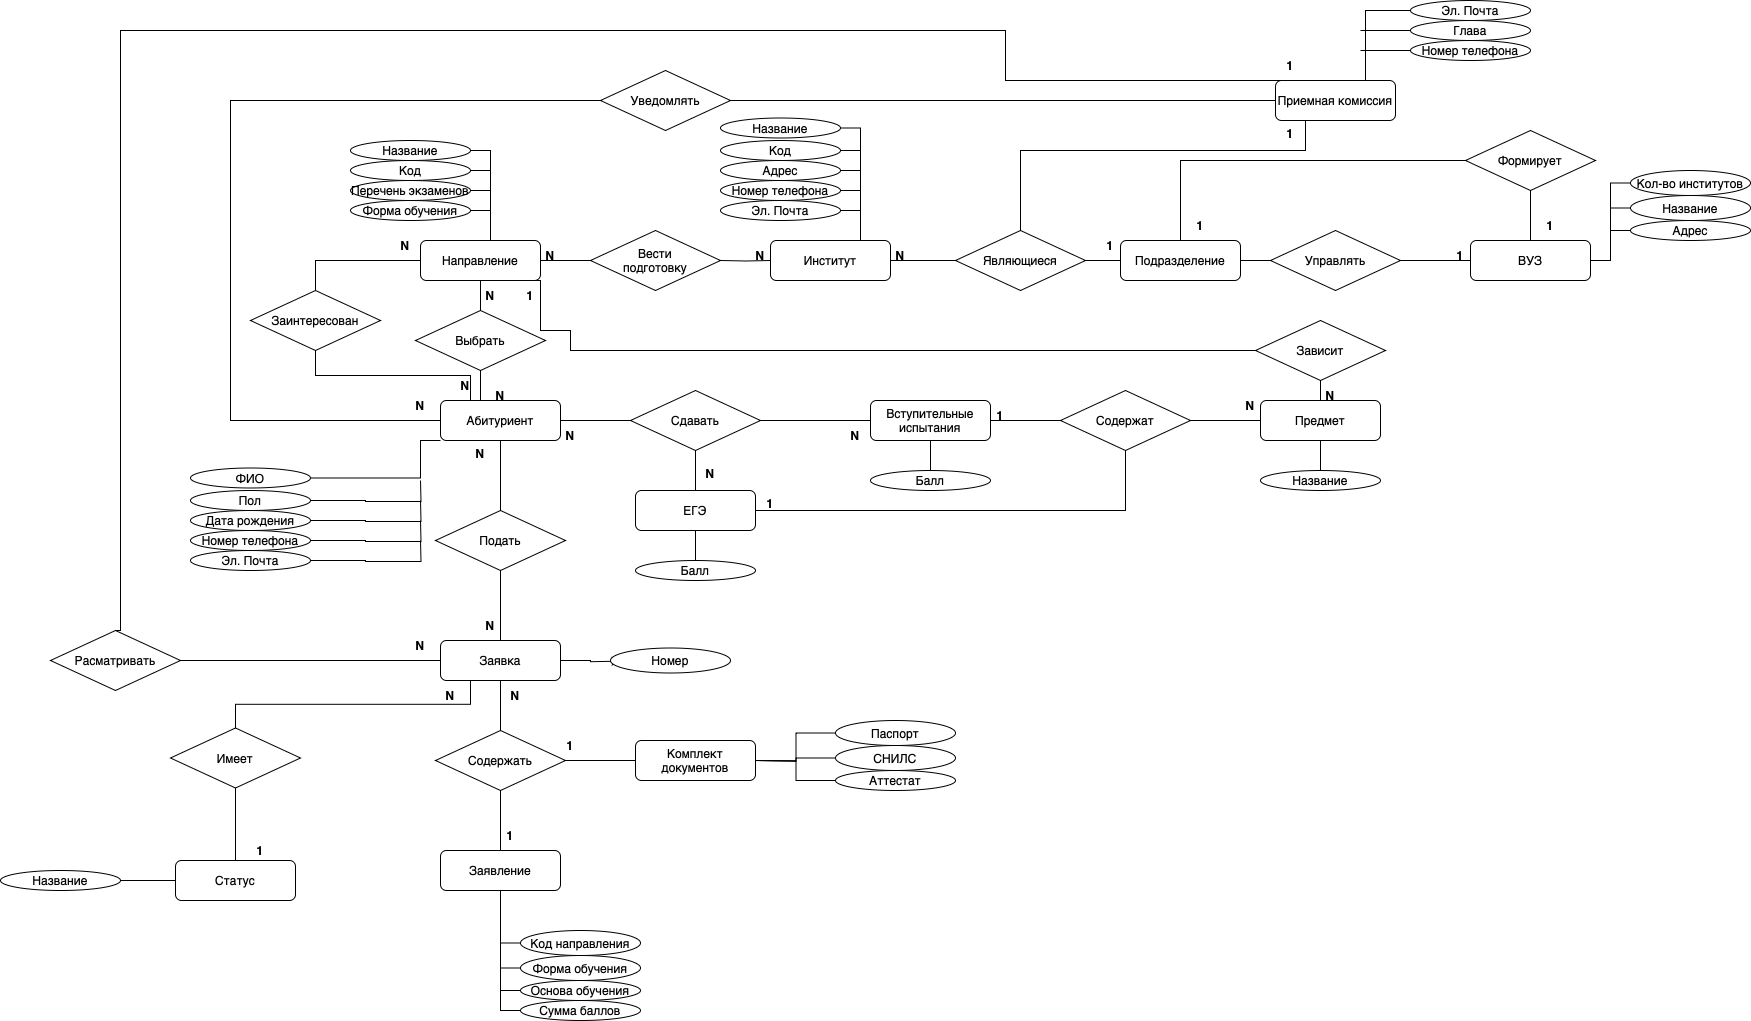
\includepdf[pages=-,landscape,fitpaper]{images/ER.pdf}

\newpage
\section{Use case}
\subsection{Уровень 1}
\begin{figure}[H]
    \centering
    
\includegraphics[width=0.7\textwidth]{images/UseCase_1.drawio.png}
    \caption{Use case диаграмма 1-го уровня}
    \label{fig:syntdiag}
\end{figure}
\textbf{Акторы}: Абитуриент, Институт, Приемная комиссия
\textbf{Триггер}: Открытие приема заявлений на обучение
\textbf{Входные данные}:
\begin{itemize}
    \item Предлагаемые институтами направления подготовки
    \item Выбор абитуриентом направление подготовки содержащиеся в институтах
    \item Набор документов
\end{itemize}
\textbf{Выходные данные}:
\begin{itemize}
    \item Начало процесса взаимодействия: выбор абитуриентом направления подготовки инициирующий последующие шаги приема.
\end{itemize}

\textbf{Основной процесс}:
\begin{enumerate}
    \item Абитуриент выбирает направление подготовки
    \item Формирование и публикация ВУЗом правил приема
    \item Вычисление баллов
    \item Публикация списков
    \item Процесс приема абитуриентов с участием подразделени (институт и приемная комиссия)
    \item Сдача ЕГЭ
    \item Сдача вступительных испытаний
    \item Подача заявки
    \item Сбор документов
    \item Зачисление бюджетников
    \item Зачисление контрактников
    \item Подготовка приказов о зачислении
    \item Выдача списка зачисленных студентов
    \item Апелляция и пересмотр результатов
    \item Выдача полного списка зачисленных студентов после апелляции
\end{enumerate}
\textbf{Альтернативный процесс}:
\begin{itemize}
    \item Из-за распространения вируса, в выбранном ВУЗ-е минимум один год, будет
проходить только заочный формат обучения. (отрицательный)
\item Министерство образования и науки отменяет лицензию ВУЗ-а. (отрицательный)
\end{itemize}
\newpage
\subsection{Уровень 2}
\begin{figure}[H]
    \centering
    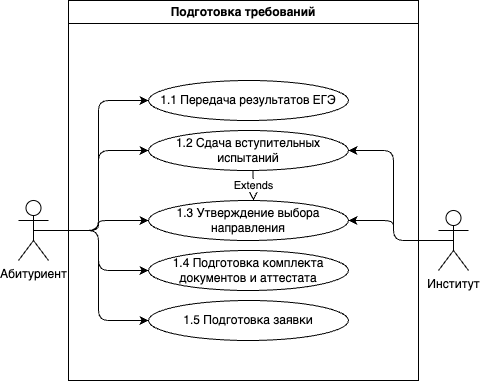
\includegraphics[width=0.7\textwidth]{images/UseCase_2.drawio.png}
    \caption{Use case диаграмма 2-го уровня}
    \label{fig:syntdiag}
\end{figure}
\textbf{Акторы}: Абитуриент, Институты
\textbf{Триггер}: Объявление о начала подачи документов
\textbf{Входные данные}:
\begin{itemize}
    \item Заявка
    \item Набор документов
    \item Баллы ЕГЭ
    \item Результаты вступительных испытаний
\end{itemize}
\textbf{Выходные данные}:
\begin{itemize}
    \item Подготовленный комплект заявки абитуриентом, включающий паспортные данные, СНИЛС, аттестат
    \item Подготовленное абитуриентом заявление содержащие форму обучения, суммы баллов, основу обучения.
\end{itemize}
\textbf{Основной процесс}:
\begin{enumerate}
    \item Абитуриент сдавший ЕГЭ подает результаты экзаменов.
    \item Абитуриент сдает вступительные испытания, зависящие от выбранного направления в определенном институте.
    \item Абитуриент готовит необходимые документы
    \item Абитуриент готовит заявление
\end{enumerate}
\textbf{Альтернативный процесс}:
\begin{itemize}
    \item Абитуриент сменил выбор направления (положительный)
    \item Один из необходимых документов абитуриента просрочен(отрицательный)
    \item Абитуриент решил поступить в зарубежный ВУЗ (положительный)
\end{itemize}
\newpage
\subsection{Уровень 3 для 1.2}
\begin{figure}[H]
    \centering
    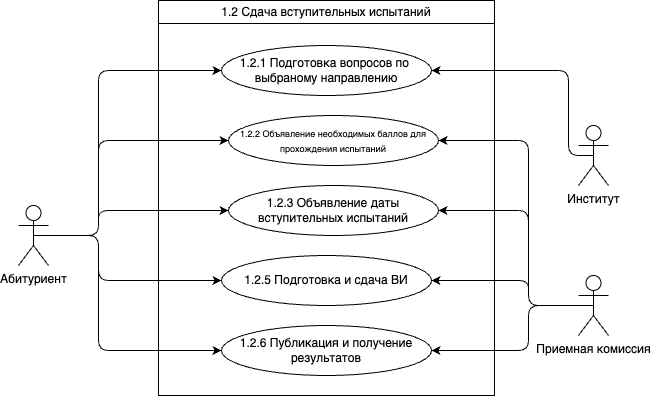
\includegraphics[width=0.7\textwidth]{images/UseCase_3_12.png}
    \caption{Use case диаграмма 3-го уровня для 1.2}
    \label{fig:syntdiag}
\end{figure}
\textbf{Акторы}: Абитуриент, Приемная комиссия, институт \\
\textbf{Триггер}: Необходимость дополнительных испытаний, помимо ЕГЭ, установленная ВУЗом.\\
\textbf{Входные данные}:
\begin{itemize}
    \item Расписание вступительных испытаний
    \item Вопросы испытаний подготовленные институтом по определенному направлению
    \item Информация о необходимых предметах
\end{itemize}
\textbf{Выходные данные}:
\begin{itemize}
    \item Результаты по соответствующим вступительным испытаниям
    \item Уведомление абитуриента
    \item Отметка о допуске/недопуске к следующему этапу процесса поступления
\end{itemize}
\textbf{Основной процесс}:
\begin{enumerate}
    \item Институты готовят вопросы испытаний по направлениям
    \item Приемная комиссия публикует и доводит до абитуриентов информацию о сроках и формате вступительных испытаний.
    \item Абитуриент знакомится с условиями и требованиями, регистрируется (при необходимости) на сдачу испытаний.
    \item Абитуриент в назначенные сроки и в установленном порядке проходит вступительное испытание: 
    \subitem Очная форма сдачи;
    \subitem Дистанционная форма.
    \item Экзамен/испытание проводится при контроле или организаторской поддержке Приемной комиссии.
    \item Результаты испытания фиксируются Приемной комиссией  
    \item Абитуриент получает уведомление о результатах
\end{enumerate}
\textbf{Альтернативный процесс}:
\begin{itemize}
    \item Абитуриент предъявил льготы для досрочного поступления без сдачи вступительных испытаний. (положительный)
\end{itemize}
\newpage
\subsection{Уровень 3 для 1.4}
\begin{figure}[H]
    \centering
    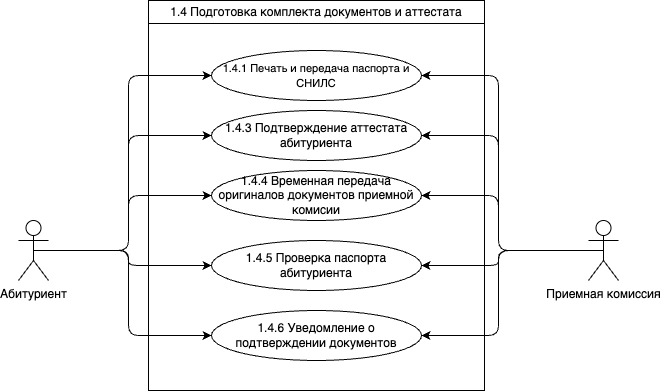
\includegraphics[width=0.7\textwidth]{images/UseCase_3_14.png}
    \caption{Use case диаграмма 3-го уровня для 1.4}
    \label{fig:syntdiag}
\end{figure} 
\textbf{Акторы}: Абитуриент, Приемная комиссия\\
\textbf{Триггер: Подтверждение приемной комиссией о допуске абитуриента до следующего этапа поступления}.\\
\textbf{Входные данные}:
\begin{itemize}
    \item Оригиналы/ копии документов удостоверяющих личность абитуриента
    \item Аттестат или иной документ об образование
    \item Перечень документов необходимых для поступления (установленные ВУЗом)
\end{itemize}
\textbf{Выходные данные}:
\begin{itemize}
    \item Сформированный комплект документов
    \item Готовность комплекта к подаче в приемную комиссию
    \item Статус о подтверждении личности абитуриента
\end{itemize}
\textbf{Основной процесс}:
\begin{enumerate}
    \item Абитуриент получает/формирует перечень необходимых для поступления документов (паспорт, СНИЛС, аттестат и т.д.).
    \item Абитуриент проверяет все сроки действия и корректность данных в документах (актуальный паспорт, подлинность аттестата).
    \item Абитуриент делает копии, заверяет их.
    \item Абитуриент готовит аттестат для передачи в ВУЗ.
    \item Абитуриент отправляет полный комплект документов приемной комиссии
    \item Приемная комиссия подтвержает личность абитуриента и его документы об образовании.
    \item Абитуриент уведомляется приемной комиссией о подтверждении личности и документов об образовании и дает допуск для следующего этапа поступления.
\end{enumerate}
\textbf{Альтернативный процесс}:
\begin{itemize}
    \item В системе проверки документов произошел сбой, всем абитуриентам было отказано в проверке документов. 
    \item Документы не смогли подтвердить на подленность.
\end{itemize}
\newpage
\subsection{Описание}
\textbf{Уровень 1}:
\begin{enumerate}
    \item Абитуриент выбирает направление подготовки, в котором он (-она) заинтересован. При успешной сдаче (сумма баллов ЕГЭ не менее пропускного балла по направлению), ЕГЭ и сдачи вступительных испытаний содержащие предметы которых зависят от выбора направления, абитуриент подает заявку содержащая в себе – комплект документов идентифицирующие личность (например: паспорт, СНИЛС), аттестат и содержит заявление, в которой прописана желаемая абитуриентом форма обучения и сумма баллов. При этом абитуриент может подать апелляцию, по ЕГЭ или вступительному испытанию. После формирования абитуриентом заявки, приемной комиссией к заявки присваивается статус, в соответствии зачисления или отказа в зачислении. После сроков апелляции ВУЗ публикует окончательный список зачисленных и отклонённых абитуриентов по их заявкам.
\end{enumerate}
\textbf{Уровень 2}:
\begin{enumerate}
    \item После того как абитуриент сдал ЕГЭ, и после чего он получил необходимые баллы, он передает результаты ЕГЭ.
    \item Если баллы за ЕГЭ не меньше минимальных требований направления,абитуриенту предлагается сдать вступительные испытания в соответствии с выбранным направлением.
    \item Абитуриент утверждает свой выбор направления, после утверждения абитуриент не сможет поменять направление в течение одного учебного года, при успешном зачислении.
    \item Абитуриент подготавливает необходимые документы, идентифицирующие личность, такие как: Паспорт, СНИЛС. И подготавливает аттестат.
    \item Абитуриент готовит заявку содержащую в себе желаемую форму обучения, и копии документов.
\end{enumerate}
\textbf{Уровень 3 для 1.1}:
\begin{enumerate}
    \item Получение абитуриентом официальных результатов ЕГЭ
    \item Вход в личный кабинет ФИПИ или получение результатов из официальной базы (при наличии соответствующего механизма)
    \item Сохранение и подготовка электронных/бумажных копий
    \item Формирование абитуриентом пакета результатов ЕГЭ для передачи
    \item Выбор необходимых предметов (согласно требованиям выбранного направления)
    \item Проверка корректности данных (ФИО, баллы, сроки действия)
    \item Передача результатов ЕГЭ в Приемную комиссию
    \item Способ передачи: личная подача, электронная система или иные регламентированные каналы
    \item Подтверждение получения документов (расписка, электронное уведомление)
    \item Проверка и регистрация результатов ЕГЭ в базе Приемной комиссии
    \item Сверка баллов и личных данных с официальными реестрами/сертификатами
    \item Регистрация баллов в информационной системе Приемной комиссии
\end{enumerate}
\textbf{Уровень 3 для 1.2}:
\begin{enumerate}
    \item Приемная комиссия проверяет финальные баллы ЕГЭ абитуриента.
    \item Приемная комиссия проверяет финальные баллы вступительных испытаний.
    \item Абитуриент выбирает одну из доступных форм обучения.
    \item Абитуриент подает комплект документов, и аттестат приемной комиссии.
    \item Абитуриент подает заявку на зачисление.
    \item Приемная комиссия утверждает основу обучения по баллам ЕГЭ.
    \item Приемная комиссия присваивает заявкам абитуриентов статусы (зачислен/ откланено)
    \item Приемная комиссия публикует список зачисленных и не зачисленных абитуриентов в открытый доступ.
\end{enumerate}
\textbf{Уровень 3 для 1.3}:
\begin{enumerate}
    \item Самостоятельный выбор направления абитуриентом
    \item Ознакомление с перечнем доступных направлений
    \item Сверка собственных ЕГЭ-баллов с требованиями (минимальными порогами)
    \item Подача заявки на выбранное направление
    \item Заполнение заявления на направление (в бумажной или электронной форме)
    \item Указание приоритетности (если подается на несколько направлений)
    \item Проверка доступных мест и соответствия баллов ЕГЭ
    \item Сверка количества вакантных мест на направлении
    \item Сравнение набранных баллов абитуриента с минимально проходными
    \item Принятие решения о зачислении/отказе по направлению
    \item При положительном решении — резервирование места (предварительное или окончательное, в зависимости от этапа)
    \item При отказе — уведомление о причинах (недостаток баллов, отсутствие мест)
    \item Уведомление абитуриента о решении
    \item Фиксация решения в информационной системе (статус Утверждено/ Отклонено)
    \item Отправка результата (e-mail, личный кабинет, звонок и т.д.)
    
\end{enumerate}
\textbf{Уровень 3 для 1.4}:
\begin{enumerate}
    \item Приемная комиссия проверяет финальные баллы ЕГЭ абитуриента.
    \item Приемная комиссия проверяет финальные баллы вступительных испытаний.
    \item Абитуриент выбирает одну из доступных форм обучения.
    \item Абитуриент подает комплект документов, и аттестат приемной комиссии.
    \item Абитуриент подает заявку на зачисление.
    \item Приемная комиссия утверждает основу обучения по баллам ЕГЭ.
    \item Приемная комиссия присваивает заявкам абитуриентов статусы (зачислен/ откланено)
    \item Приемная комиссия публикует список зачисленных и не зачисленных абитуриентов в открытый доступ.
\end{enumerate}
\textbf{Уровень 3 для 1.5}:
\begin{enumerate}
    \item Формирование пакета документов для идентификации личности
    \item Сбор необходимых документов (паспорт, СНИЛС и т.д.)
    \item Проверка актуальности и корректности (срок действия паспорта, наличие всех страниц)
    \item Подготовка аттестата или иного документа об образовании
    \item Сверка соответствия уровня образования (аттестат о среднем общем, диплом о среднем проф. и пр.)
    \item Уточнение необходимости оригинала или заверенной копии
    \item Оформление заявления абитуриента
    \item Указание желаемой формы обучения (очная/заочная/очно-заочная)
    \item Указание суммы баллов по ЕГЭ/ВИ (вступительным испытаниям)
    \item Подпись/электронная подпись заявления
    \item Подача сформированной заявки (пакета документов) в Приемную комиссию
    \item Определение канала подачи (лично, через электронный портал, почта)
    \item Регистрация заявки в журнале/информационной системе
    \item Присвоение заявке статуса в системе Приемной комиссии
    \item Первичная проверка корректности и полноты документов (статус "На проверке")
    \item При соответствии всем требованиям – присвоение статуса "Принято к конкурсу" и уведомление абитуриента
\end{enumerate}
\newpage
\section{BPM-диаграмма №1}
На странице 24 представлена дигаграмма бизнес процессов. 
В качестве анализируемого процесса, был выбран процесс подачи документов абитуриентом в приемную комиссию.
\subsection{Описание}
Институт считает свободные места по своим направлениям, после открывает набор абитуриентов под количество мест, сообщая об этом Приемной комиссии инициируя процесс (процесс института завершен корректно). 

Приемная комиссия, публично оповещает о открытие набора абитуриентов, после некоторого времени, приемная комиссия, оповещает о начале сбора документов который инициирует процесс подготовки документов абитуриентом. Приемная комиссия начинает прием документов. 

Абитуриент подготавливает паспорт, если абитуриент - иностранец, он делает перевод паспорта, после идет подготовка аттеста, если аттестат - иностранный, абитуриент делает перевод аттестата. Если абитуриент гражданин РФ, то он подготавливает СНИЛС. Иностранный абитуриент, должен наториально заверить перевод документов. Иностранному абитуриенту, нужно время, на ожидание наториального заверения. После если у абитуриента есть льготы, он(-а), готовят их. Либо сразу передают комплект документов. Однако у абитуриента могут возьникнуть непредвиденные обстоятельства по причинам который он(-она) не будет подавать документы (процесс завершен), или же абитуриент не успел подать документы в срок сдачи (процесс завершен). При успешной подачи документов, привемная комиссия дает заявление на подтверждение согласия на временную передачу документов. В этом случае абитуриент или приемная комиссия могут по собственной или иной причине отказатся от процедуры (процесс завершен). Если же абитуриент подписывает заявление, приемная комиссия передает документ подтверждающий временую передачу документов. После чего абитуриент ожидает уведомления. 
Приемная комиссия поверяет документы, аттестат и при наличии льготы. После либо уведомляет абитуриента о успешном принятии документов, либо об отказе от принятия документов. После отказа - абитуриенту возвращаются все поданные им документы. При успешном принятии документов, абитуриенту возвращаются паспорт, СНИЛС. 
Абитуриент получает уведомление. Абитуриент получает документы. Абитуриент завершает процесс (завершение процесса корректно).
После срока принятия подачи документов абитуриентов, приемная комиссия завершает свой процесс по принятию документов (завершение процесса корректно).
    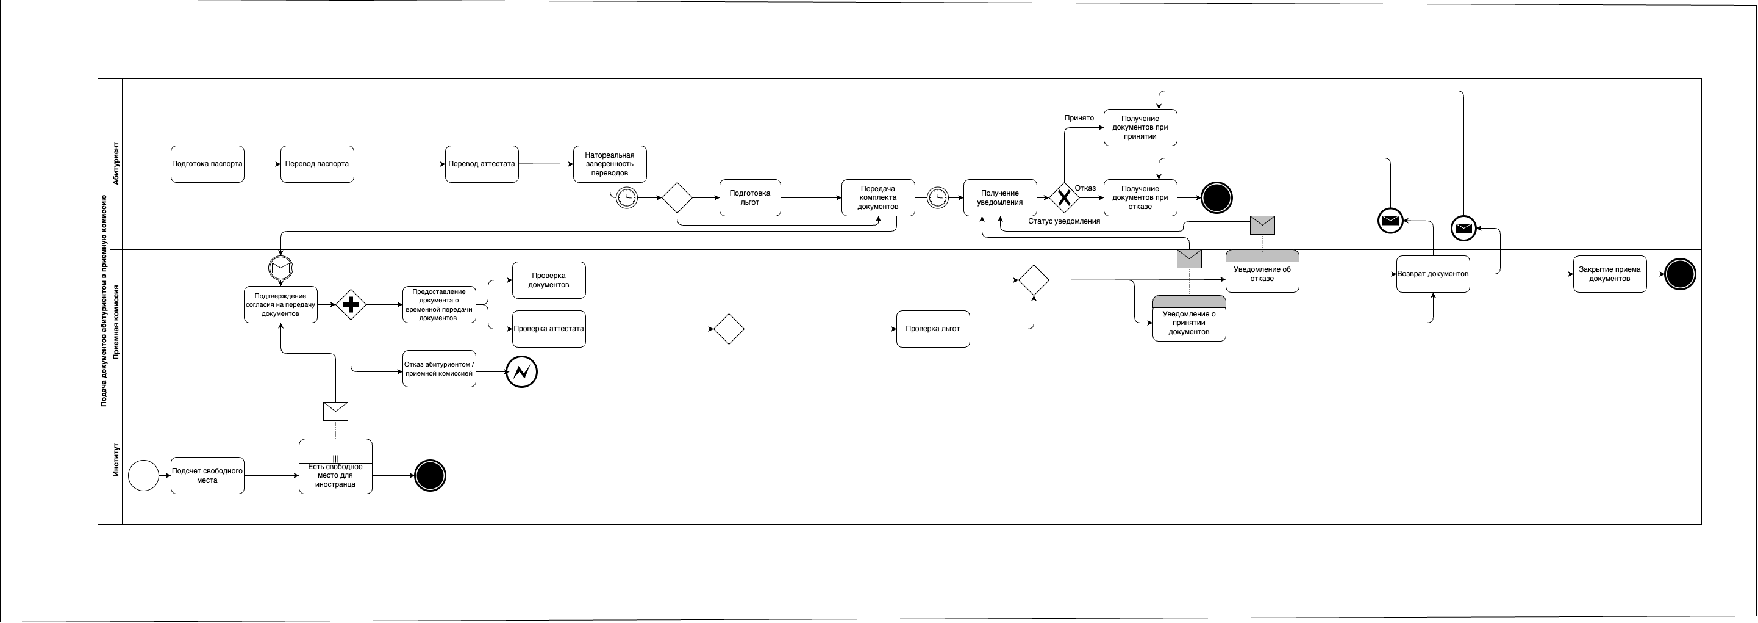
\includepdf[pages=-,landscape,fitpaper]{images/BPM_1.pdf}
\newpage
\section{BPM-диаграмма №2}
На странице 26 представлена диаграмма бизнес процесса, не относящаяся к основному процессу. 
В качестве анализируемого процесса был выбран процесс: Оформление пропуска студента.
\subsection{Описание}
Студент пишет заявление на получение пропуска и инициирует процесс пропускного отдела пропускной отдел пишет заявление на получение данных в деканат. Заявление на получение данных студента принимает деканат, проводит поиск данных студента по документам если студенты не оказалось в базе процесс завершается с ошибкой, если уже студент найден то происходит проверка статуса обучения если формируется отказ от заявления далее происходит пояснение отказа либо студент в академическом отпуске, либо студент отчислен. Если же заявление подтверждается то отправляется письмо от проверки статуса заявления далее пропускной отдел либо сообщает об отказе, либо начинает подготовку пропуска. После готовности сообщает студенту. Студент получает извещение далее студент приходит в отделение. Отдел по пропускам выдает документы студенту. Студент получает документы процесс завершается.
    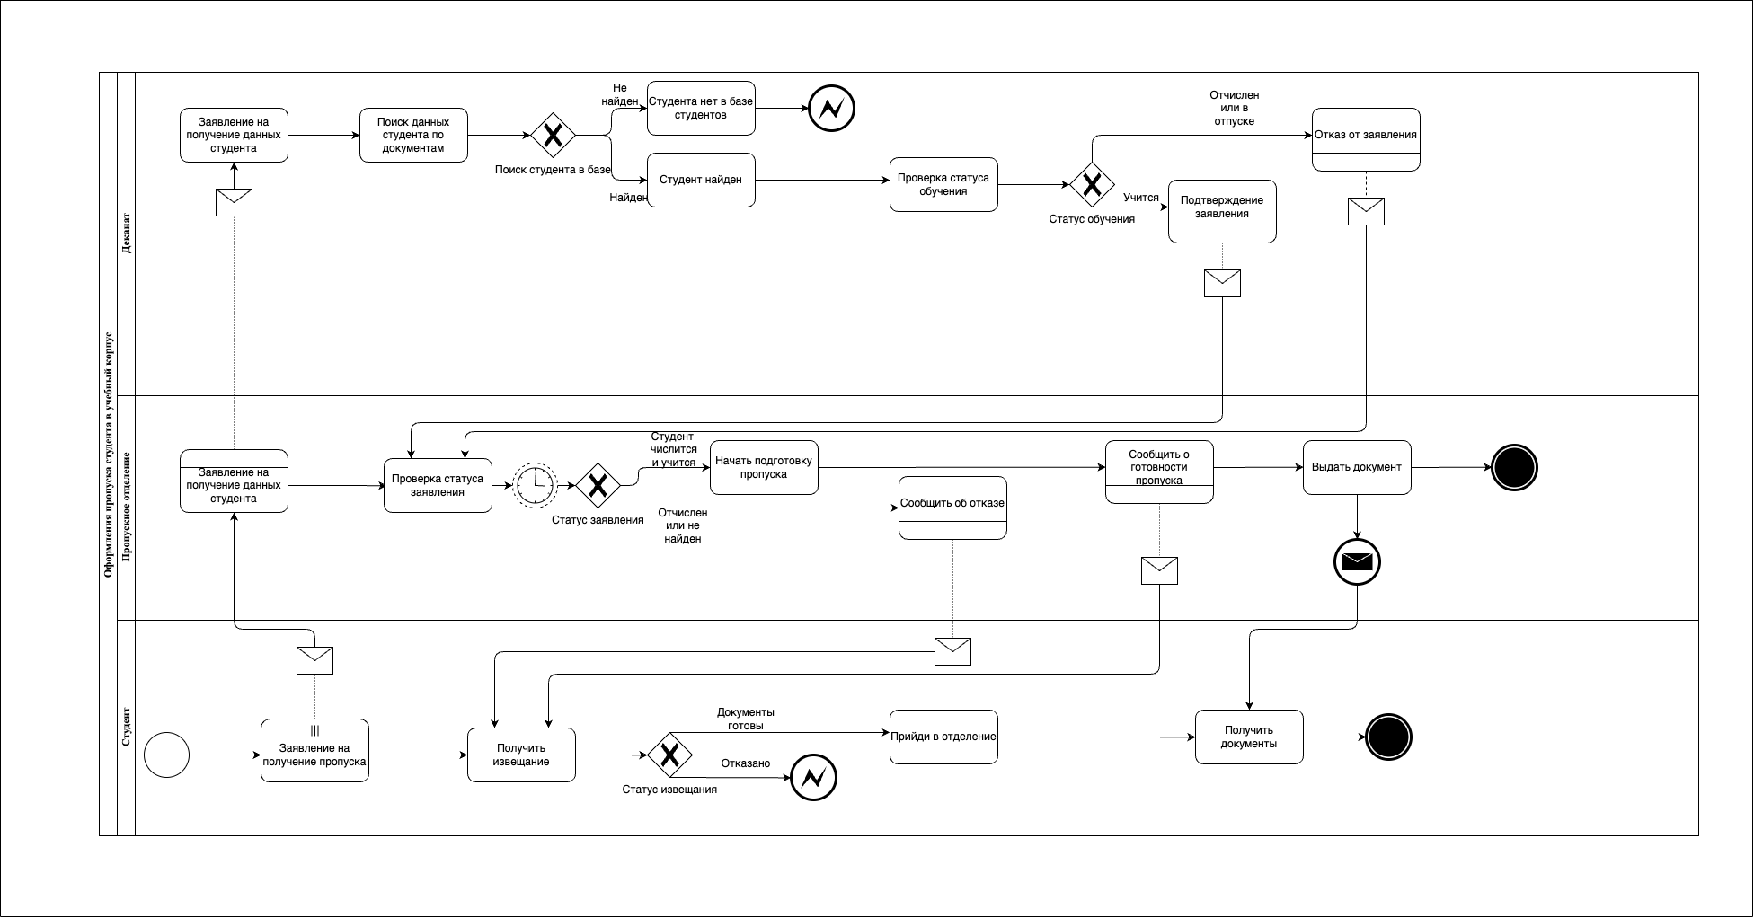
\includepdf[pages=-,landscape,fitpaper]{images/BPM_2.pdf}
\newpage
\section{Описание экранных форм}
\subsection{Цель создания форм}
\begin{itemize}
    \item Автоматизация пресса обслуживания клиента;
    \item Формализация общения между участниками процесса, во избежание ошибок, вызванных человеческим фактором.
\end{itemize}
\subsection{Описание экранной формы}
Абитуриент подает заявление на выбор направления в приемную комиссию.
Может произойти три исхода:
\begin{enumerate}
    \item Заявление написано неверно (Приемная комиссия отдает заявление с просьбой переделать его) $\Rightarrow$ абитуриент
    вынужден подать апелляции. 
    \item Заявление написано верно (Приемная комиссия принимает заявление и уведомляет абитуриента) 
    \item В выбранном направление закончились места (Приемная комиссия уведомляет абитуриента и возвращает заявление с альтернтивой)
\end{enumerate}
При успешном подачи заявления, приемная комиссия регистрирует заявление в электронном журнале. 
\newpage
\subsection{Граф связи форм}
Граф связи форм представлен на рисунке №5.
\begin{figure}[H]
    \centering
    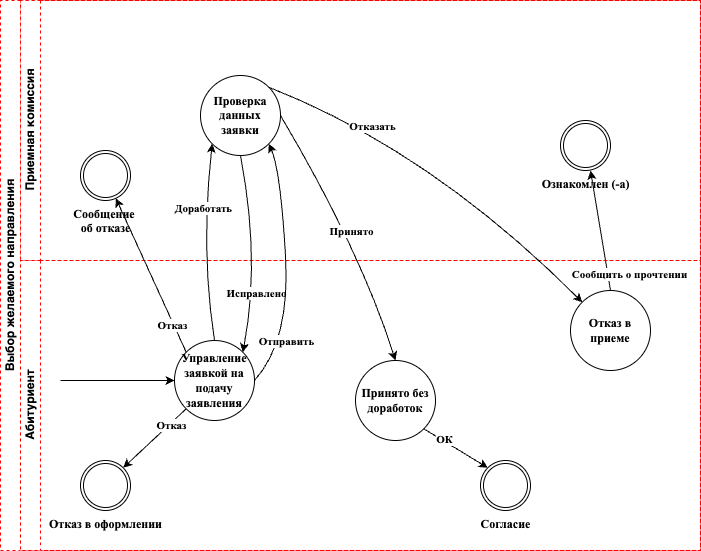
\includegraphics[width=0.9\textwidth]{images/GraphProject.png}
    \caption{Граф связи форм}
    \label{fig:syntdiag}
\end{figure}

\newpage
\subsection{JSON-формат для хранения данных}
\subsubsection{Базовый JSON}
\begin{lstlisting}[language=json,caption={Bazovyi JSON format zayavki},label={lst:json-base}]
{
  // Osnovnaya informaciya o zayavke
  "application": {
    "id": null,                    // UUID zayavki
    "version": "1.0",             // Versiya formata
    "createdAt": null,            // Data i vremya sozdaniya (ISO 8601)
    "updatedAt": null,            // Data i vremya poslednego obnovleniya (ISO 8601)
    "attempts": 0,                // Kolichestvo popytok podachi
    "state": "draft",            // Tekushee sostoyanie
    "direction": {
      "code": null,              // Kod napravleniya
      "name": null,              // Nazvanie napravleniya
      "institute": null,         // Institut
      "form": null,              // Forma obucheniya (full-time, part-time)
      "basis": null,             // Osnova obucheniya (budget, contract)
      "priority": null           // Prioritet napravleniya
    }
  },

  // Informaciya ob abituriente
  "applicant": {
    "personal": {
      "surname": null,           // Familiya
      "name": null,              // Imya
      "lastName": null,          // Otchestvo (opcionalno)
      "birthDate": null,         // Data rozhdeniya (YYYY-MM-DD)
      "email": null,             // Email dlya svyazi
      "phone": null              // Telefon dlya svyazi
    },
    "address": {
      "country": null,           // Strana
      "city": null,              // Gorod
      "street": null,            // Ulitsa
      "house": null,             // Nomer doma
      "apartment": null          // Nomer kvartiry (opcionalno)
    }
  },

  // Dokumenty abiturienta
  "documents": {
    "passport": {
      "series": null,            // Seriya pasporta
      "number": null,            // Nomer pasporta
      "issueDate": null,         // Data vydachi (YYYY-MM-DD)
      "issuePlace": null,        // Mesto vydachi
      "original": null,          // Put k originalu pasporta
      "translation": null        // Put k perevodu pasporta (dlya inostrancev)
    },
    "snils": {
      "number": null,            // Nomer SNILS
      "file": null               // Put k SNILS
    },
    "education": {
      "type": null,              // Tip obrazovaniya (school, college, university)
      "document": {
        "type": null,            // Tip dokumenta (attestat, diploma)
        "number": null,          // Nomer dokumenta
        "issueDate": null,       // Data vydachi (YYYY-MM-DD)
        "issuePlace": null,      // Mesto vydachi
        "original": null,        // Put k originalu dokumenta ob obrazovanii
        "translation": null      // Put k perevodu dokumenta (dlya inostrancev)
      },
      "graduationYear": null,    // God okonchaniya
      "averageScore": null       // Sredniy ball
    },
    "photos": [],                // Massiv putej k fotografiyam
    "additional": []             // Massiv putej k dopolnitelnym dokumentam
  },

  // Rezultaty ekzamenov
  "scores": {
    "ege": {
      "russian": null,           // Ball po russkomu yazyku
      "math": null,              // Ball po matematike
      "physics": null,           // Ball po fizike
      "informatics": null,       // Ball po informatike
      "english": null            // Ball po angliyskomu yazyku
    },
    "entrance": {
      "subject1": null,          // Ball po pervomu vstupitelnomu ispytaniyu
      "subject2": null           // Ball po vtoromu vstupitelnomu ispytaniyu
    },
    "total": null                // Obshiy ball
  },

  // Status i proverka zayavki
  "status": {
    "current": "draft",          // Tekuschiy status
    "previous": null,            // Predyduschiy status
    "lastUpdate": null,          // Vremya poslednego obnovleniya statusa
    "nextDeadline": null,        // Sleduyuschiy deadline
    "isFinal": false,            // Finalny li status
    "review": {
      "reviewer": {
        "id": null,              // ID proveryayuschego
        "name": null,            // FIO proveryayuschego
        "role": null             // Rol proveryayuschego
      },
      "comments": [],            // Massiv kommentariev komissii
      "decisions": [],           // Massiv resheniy komissii
      "verificationResults": {
        "documents": {
          "passport": false,     // Rezultat proverki pasporta
          "education": false,    // Rezultat proverki dokumenta ob obrazovanii
          "snils": false         // Rezultat proverki SNILS
        },
        "scores": {
          "ege": false,          // Rezultat proverki ballov EGE
          "entrance": false      // Rezultat proverki vstupitelnyh ispytaniy
        }
      }
    }
  }
}
\end{lstlisting}
\newpage
\subsubsection{Пример JSON с историей заявки}
\begin{lstlisting}[language=json,caption={JSON с историей заявки},label={lst:json-history}]
{
  // Sistemnaya informaciya
  "id": "d9a87c9e-4b1d-48b6-8f94-443d2c098721",
  "version": "1.0",
  "createdAt": "2025-05-02T10:15:00+03:00",
  "updatedAt": "2025-05-06T09:13:19+03:00",
  "attempts": 2,
  "state": "accepted_by_commission",
  "metadata": {
    "source": "web",
    "ip": "192.168.1.1",
    "userAgent": "Mozilla/5.0...",
    "sessionId": "sess123456"
  },

  // Informaciya o zayavitele i ego dokumentah
  "applicant": {
    "personal": {
      "surname": "Salimli",
      "name": "Ayzek",
      "lastName": "Salimli",
      "birthDate": "2000-01-01",
      "email": "salimli.am@edu.spbstu.ru",
      "phone": "+7 (999) 123-45-67"
    },
    "address": {
      "country": "Russia",
      "city": "Saint-Petersburg",
      "street": "Polytechnicheskaya",
      "house": "29",
      "apartment": "123"
    },
    "documents": {
      "passport": {
        "series": "4012",
        "number": "987654",
        "issueDate": "2020-01-01",
        "issuePlace": "Saint-Petersburg",
        "original": "passport.pdf",
        "translation": null
      },
      "snils": {
        "number": "123-456-789 00",
        "file": "snils.pdf"
      },
      "education": {
        "type": "school",
        "document": {
          "type": "attestat",
          "number": "123456",
          "issueDate": "2024-06-25",
          "issuePlace": "134",
          "original": "attestat.pdf",
          "translation": null
        },
        "graduationYear": "2024",
        "averageScore": 4.8
      },
      "photos": ["photo1.jpg", "photo2.jpg"],
      "additional": []
    }
  },

  // Informaciya o zayavke i rezultatah
  "application": {
    "direction": {
      "code": "02.03.01",
      "name": "Mathematics and Computer Science",
      "institute": "IKNK",
      "form": "full-time",
      "basis": "budget",
      "priority": 1
    },
    "scores": {
      "ege": {
        "russian": 85,
        "math": 90,
        "physics": 88,
        "informatics": 92,
        "english": 0
      },
      "entrance": {
        "subject1": 95,
        "subject2": 90
      },
      "total": 355
    }
  },

  // Status i proverka zayavki
  "status": {
    "current": "accepted_by_commission",
    "previous": "in_review",
    "lastUpdate": "2025-05-06T09:13:19+03:00",
    "nextDeadline": "2025-05-20T23:59:59+03:00",
    "isFinal": false,
    "review": {
      "reviewer": {
        "id": "rev123",
        "name": "Salimli Ayzek",
        "role": "expert"
      },
      "comments": [
        {
          "timestamp": "2025-05-03T08:21:54+03:00",
          "text": "Please provide the original attestat",
          "type": "request"
        }
      ],
      "decisions": [
        {
          "timestamp": "2025-05-03T08:21:54+03:00",
          "type": "revision",
          "reason": "Missing original attestat"
        },
        {
          "timestamp": "2025-05-06T09:13:19+03:00",
          "type": "accept",
          "reason": "All documents are in order"
        }
      ],
      "verificationResults": {
        "documents": {
          "passport": true,
          "education": true,
          "snils": true
        },
        "scores": {
          "ege": true,
          "entrance": true
        }
      }
    }
  },

  // Uvedomleniya i istoriya
  "notifications": {
    "sent": [
      {
        "type": "email",
        "timestamp": "2025-05-03T08:22:00+03:00",
        "subject": "Revision Required",
        "status": "delivered"
      },
      {
        "type": "email",
        "timestamp": "2025-05-06T09:15:00+03:00",
        "subject": "Application Accepted",
        "status": "delivered"
      }
    ],
    "received": []
  },
  "history": [
    {
      "event": "created",
      "timestamp": "2025-05-02T10:15:00+03:00",
      "actor": "applicant",
      "details": "New application created"
    },
    {
      "event": "submitted",
      "timestamp": "2025-05-02T10:46:33+03:00",
      "actor": "applicant",
      "details": "First submission attempt"
    },
    {
      "event": "revision_requested",
      "timestamp": "2025-05-03T08:21:54+03:00",
      "actor": "reviewer",
      "details": "Request for revision of documents"
    },
    {
      "event": "resubmitted",
      "timestamp": "2025-05-05T11:07:02+03:00",
      "actor": "applicant",
      "details": "Second submission attempt"
    },
    {
      "event": "accepted",
      "timestamp": "2025-05-06T09:13:19+03:00",
      "actor": "reviewer",
      "details": "Application accepted by commission"
    }
  ]
}
\end{lstlisting}

\subsubsection{Описание состояний}
\begin{description}
  \item[draft] Черновик - начальное состояние заявки. Абитуриент заполняет данные, но еще не отправил на проверку.
  \item[in\_review] На проверке - заявка отправлена на проверку в приемную комиссию.
  \item[revision\_required] Требуется доработка - приемная комиссия запросила доработку заявки.
  \item[accepted\_by\_commission] Принята комиссией - заявка принята приемной комиссией.
  \item[rejected] Отклонена - заявка отклонена приемной комиссией.
  \item[final\_acceptance] Подтверждено зачисление - абитуриент подтвердил согласие на зачисление.
  \item[cancelled\_by\_applicant] Отменена абитуриентом - абитуриент отменил заявку.
  \item[completed] Завершена - заявка успешно завершена (зачисление).
  \item[expired] Истекла - заявка истекла по сроку.
\end{description}

\paragraph{Преимущества}
\begin{itemize}
  \item Весь маршрут заявки прозрачен и однозначно воспроизводим.  
  \item Счётчик \verb|attempts| защищает комиссию от бесконечных правок.  
  \item Терминальные состояния (\textbf{s1, s2, s5, s7}) блокируют дальнейшие переходы, 
        что упрощает реализацию DFA в коде: проверяется лишь признак \verb|state in final|.
\end{itemize}

\newpage
\subsection{Форма «Управление заявкой на подачу заявления»}
\begin{table}[H]
\caption{Экран «Управление заявкой» — заполняется абитуриентом}
\renewcommand{\arraystretch}{1.2}
\begin{tabular}{|p{0.28\linewidth}|p{0.66\linewidth}|}
\hline
\textbf{Раздел} & \textbf{Описание} \\ \hline
\textbf{Назначение} &
Позволяет абитуриенту создать или доработать заявку на поступление и отправить её на проверку приёмной комиссии. \\ \hline

\textbf{Основные поля} &
\begin{enumerate}
  \item Личные данные (паспорт, Ф.\,И.\,О., дата рождения)\,*  
  \item Контакты (телефон, e-mail)\,*  
  \item Желаемое направление подготовки\,*  
  \item Согласие на обработку ПДн (чекбокс)\,*  
  \item Прикрепляемые файлы: паспорт, селфи, документы об образовании
\end{enumerate} «\,*» — обязательные поля. \\ \hline

\textbf{Кнопки действий} &
\begin{itemize}
  \item \emph{«Отправить»} — сохраняет JSON, увеличивает счётчик \texttt{attempts} и передаёт заявку комиссии.
  \item \emph{«Отказаться от оформления»} — очищает JSON и завершает процесс (заявка не создаётся).
  \item \emph{«Отправить отказ в комиссию»} — формирует запись об отказе и закрывает процесс.
  \item \emph{«Сохранить черновик»} — локальное сохранение без увеличения \texttt{attempts}.
\end{itemize} \\ \hline

\textbf{Динамика формы} &
Если заявка вернулась на доработку, возле проблемных полей отображаются комментарии комиссии; после исправления активируется кнопка «Исправлено → Отправить». \\ \hline
\end{tabular}
\end{table}

\subsection{Форма «Проверка данных заявки»}
\begin{table}[H]
\caption{Экран «Проверка данных заявки» — рабочее место сотрудника приёмной комиссии}
\renewcommand{\arraystretch}{1.2}
\begin{tabular}{|p{0.28\linewidth}|p{0.66\linewidth}|}
\hline
\textbf{Раздел} & \textbf{Описание} \\ \hline
\textbf{Назначение} &
Позволяет эксперту приёмной комиссии просмотреть сведения, присланные абитуриентом, принять одно из решений и зафиксировать его в JSON-записи заявки. \\ \hline

\textbf{Ключевые элементы интерфейса} &
\begin{itemize}
  \item Блок сведений о попытке: \emph{ID заявки}, \emph{номер попытки}, \emph{дата/время отправки}, \emph{общее число попыток}.
  \item Карточка абитуриента: Ф.\,И.\,О., дата рождения, контактные данные.
  \item Карточка документов: сканы паспорта, селфи, аттестат/диплом (кнопка «Скачать всё ZIP»).
  \item Карточка автоматической проверки: статусы «ОК» / «Ошибка».
  \item Комментарий эксперта: многострочное поле для свободного текста (обязательное при отказе или доработке).
  \item Кнопки действий:
        \begin{itemize}
          \item \emph{«Доработать»} — возвращает заявку абитуриенту со статусом «Требуется доработка».
          \item \emph{«Принято»} — переводит заявку в статус «Принята приёмной комиссией».
          \item \emph{«Отказать навсегда»} — окончательный отказ, заявка закрыта.
        \end{itemize}
\end{itemize} \\ \hline

\textbf{Бизнес-правила} &
\begin{enumerate}
  \item Кнопка «Принято» активна только при отсутствии критических ошибок автопроверки.
  \item Отрицательное решение («Доработать» или «Отказать навсегда») требует заполненного комментария.
  \item При любом решении система обновляет поле \texttt{state} в JSON, сохраняет дату, Ф.\,И.\,О. сотрудника и ЭЦП.
\end{enumerate} \\ \hline

\textbf{Ошибки и уведомления} &
Верхний баннер: \emph{зелёный} — «Заявка принята»; \emph{жёлтый} — «Отправлена на доработку»; \emph{красный} — «Заявка отклонена». \\ \hline
\end{tabular}
\end{table}

\subsection{Форма «Согласие на зачисление»}
\begin{table}[H]
\caption{Экран «Согласие на зачисление»}
\renewcommand{\arraystretch}{1.2}
\begin{tabular}{|p{0.28\linewidth}|p{0.66\linewidth}|}
\hline
\textbf{Раздел} & \textbf{Описание} \\ \hline
\textbf{Назначение} &
Получить от абитуриента окончательное согласие на зачисление после положительного решения комиссии. \\ \hline

\textbf{Содержимое экрана} &
\begin{itemize}
  \item Текст оферты-согласия (PDF доступен для скачивания).
  \item Информация о решении комиссии: номер заявки, дата принятия, направление.
  \item Способ подтверждения: 
        \begin{itemize}
          \item Подпись квалифицированной ЭЦП (виджет КриптоПРО) \emph{или}
          \item Чекбокс «Согласен» + ввод SMS-кода.
        \end{itemize}
\end{itemize} \\ \hline

\textbf{Кнопка} &
\emph{«ОК»} — подписывает JSON, фиксирует согласие и делает заявку недоступной для дальнейшего редактирования. \\ \hline
\end{tabular}
\end{table}

\subsection{Форма «Сообщение об отказе»}
\begin{table}[H]
\caption{Экран «Сообщение об отказе»}
\renewcommand{\arraystretch}{1.2}
\begin{tabular}{|p{0.28\linewidth}|p{0.66\linewidth}|}
\hline
\textbf{Раздел} & \textbf{Описание} \\ \hline
\textbf{Назначение} &
Отобразить абитуриенту официальный отказ, указать причину и предоставить возможность подтвердить факт ознакомления. \\ \hline

\textbf{Элементы экрана} &
\begin{itemize}
  \item Красный баннер «Заявка отклонена».
  \item Таблица параметров: дата и время отказа, номер заявки, число попыток, Ф.\,И.\,О. ответственного сотрудника.
  \item Блок причины отказа: свободный текст (до 2000 символов).
  \item Скан официального письма (PDF с печатью и подписью).
\end{itemize} \\ \hline

\textbf{Кнопка} &
\emph{«Ознакомлен»} — фиксирует отметку \texttt{applicant\_read = true} в JSON и закрывает доступ к редактированию. \\ \hline
\end{tabular}
\end{table}

\newpage
\section{Эскизы экранных форм}
Правило для различия элементов интерфейса:
\begin{itemize}
  \item для редактируемых полей используется белый фон и иконка-карандаш рядом;
  \item для нередактируемых полей используется серый фон;
  \item для баннеров используется красный (отказан), зелёный (принят) или жёлтый (основные формы);
  \item для титульных надписей используется синий фон;
  \item кнопки имеют выпуклую форму и: \begin{itemize}
    \item для действий: подтверждения, ознакомления, принятия, просмотра попыток - зеленый фон;
    \item для действий: удаления, очистки, отказа, отказа в оформлении - красный фон;
    \item для действий: скачать файл - голубой фон;
    \item для действий: сохранить черновик - темно-синий фон.
  \end{itemize}
\end{itemize}

\subsection{Форма «Управление заявкой на подачу заявления»}
\begin{figure}[H]
\centering
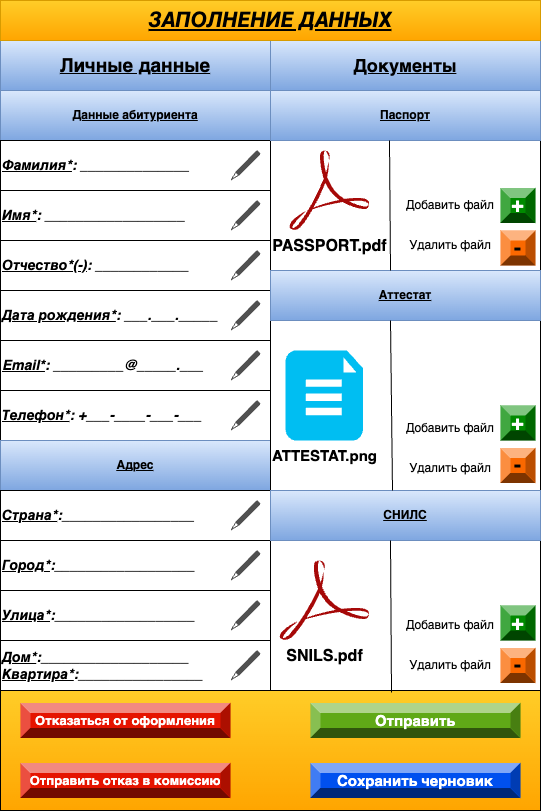
\includegraphics[width=0.8\textwidth]{images/FINAL_ABIII.png}
\caption{Эскиз формы «Управление заявкой на подачу заявления»}
\end{figure}

\subsection{Форма «Проверка данных заявки»}
\begin{figure}[H]
\centering
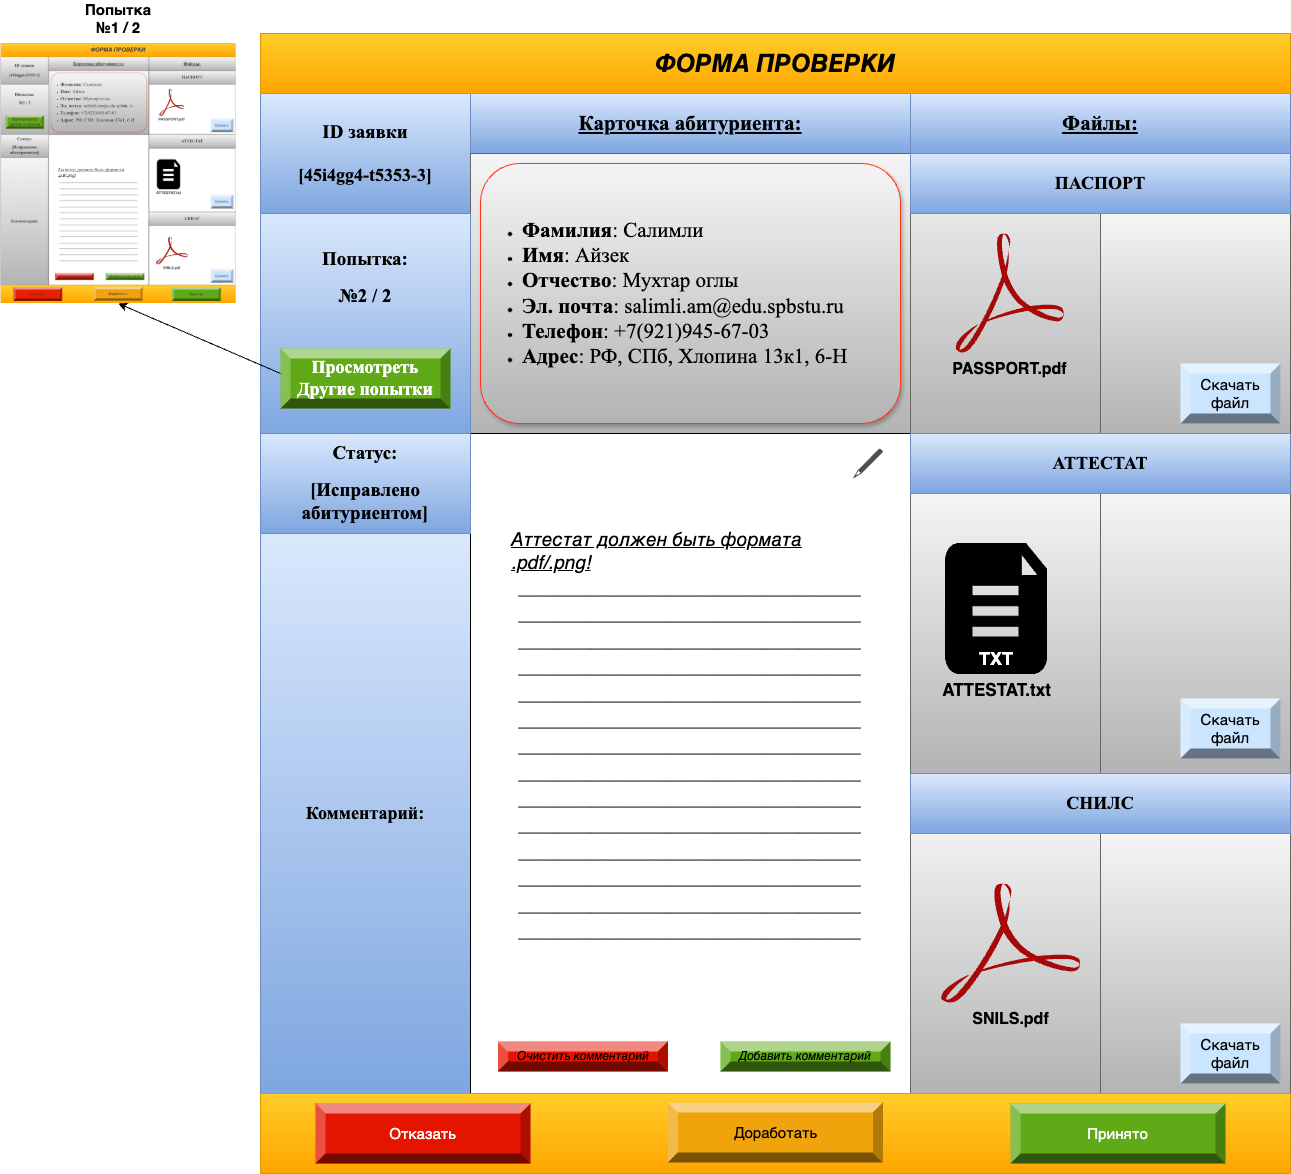
\includegraphics[width=0.8\textwidth]{images/Kommissiya.png}
\caption{Эскиз формы «Проверка данных заявки»}
\end{figure}

\subsection{Форма «Согласие»}
\begin{figure}[H]
\centering
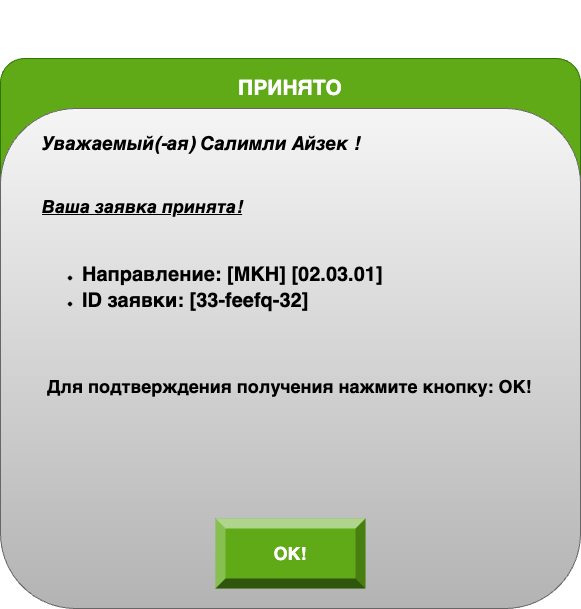
\includegraphics[width=0.8\textwidth]{images/Prinyato.png}
\caption{Эскиз формы «Согласие»}
\end{figure}

\subsection{Форма «Требуется доработка»}
\begin{figure}[H]
\centering
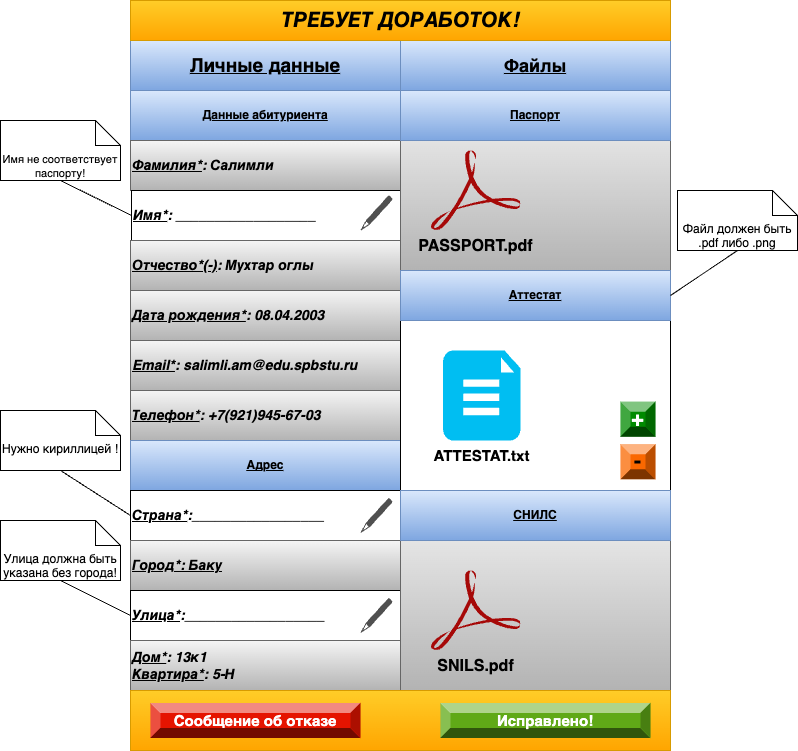
\includegraphics[width=1.0\textwidth]{images/editpls.png}
\caption{Эскиз формы «Требуется доработка»}
\end{figure}

\subsection{Форма «Откланено»}
\begin{figure}[H]
\centering
\includegraphics[width=0.8\textwidth]{images/otkaz.png}
\caption{Эскиз формы «Откланено»}
\end{figure}

\newpage
\section*{Заключение}
\addcontentsline{toc}{section}{Заключение}
В результате выполнения работы процесс проведения выставок для оценки породности собак был формализован при помощи текстового описания, ER-диаграммы, BPM-диаграмм, Use Case-диаграмм и описаний.
    \\
Построенная ER-диаграмма содержит 11 сущностей, 31 атрибута и 13 связей.
Все Use Case диаграммы суммарно содержат 18 прецедентов и 3 акторов. Для всех прецедентов были составлены Use Case описания. Были построены BPM-диаграммы для одного из подпроцессов основного процесса, а так же BPM для другого процесса. Так же были построены: детализированный граф состояний процесса подачи заявления с полным описанием вершин и условий переходов, спроектированы текстовые макеты экранных форм для ввода персональных данных абитуриента и для ручной проверки комиссии, а также выполнена спецификация формата обмена данными в виде JSON (разработан базовый шаблон и пример заполнения). 
\newpage
\section*{Список источников}
\addcontentsline{toc}{section}{Список источников}
\begin{enumerate}
    \item ГРИММОН А. BPMN. Системный подход к моделированию бизнес‑процессов. – СПб.: Питер, 2013. – 384 с.
    \item БЛАГОВЕЩЕНСКИЙ А. С., КУРЦОВ Д. А. UML 2.0. Практическое руководство. – М.: ДМК Пресс, 2007. – 528 с.
\end{enumerate}
\end{document}